\documentclass[10pt, conference, compsocconf]{IEEEtran}

\usepackage{cite}
\ifCLASSINFOpdf
  \usepackage[pdftex]{graphicx}
  % declare the path(s) where your graphic files are
  \graphicspath{{../pdf/}{../jpeg/}}
  % and their extensions so you won't have to specify these with
  % every instance of \includegraphics
  \DeclareGraphicsExtensions{.pdf,.jpeg,.png}
\else
  % or other class option (dvipsone, dvipdf, if not using dvips). graphicx
  % will default to the driver specified in the system graphics.cfg if no
  % driver is specified.
  \usepackage[dvips]{graphicx}
  % declare the path(s) where your graphic files are
  \graphicspath{{../eps/}}
  % and their extensions so you won't have to specify these with
  % every instance of \includegraphics
  \DeclareGraphicsExtensions{.eps}
\fi

% *** FLOAT PACKAGES ***
%
\usepackage{fixltx2e}
% fixltx2e, the successor to the earlier fix2col.sty, was written by
% Frank Mittelbach and David Carlisle. This package corrects a few problems
% in the LaTeX2e kernel, the most notable of which is that in current
% LaTeX2e releases, the ordering of single and double column floats is not
% guaranteed to be preserved. Thus, an unpatched LaTeX2e can allow a
% single column figure to be placed prior to an earlier double column
% figure. The latest version and documentation can be found at:
% http://www.ctan.org/tex-archive/macros/latex/base/

\usepackage{url}
\usepackage[utf8]{inputenc}
\usepackage[T1]{fontenc}
%\usepackage[colorinlistoftodos,textsize=footnotesize,textwidth=1cm]{todonotes}
% \usepackage[disable]{todonotes}
\usepackage{todonotes}
\usepackage{booktabs}
\usepackage{multirow}
\usepackage{array}
\usepackage[cmex10]{amsmath}
\usepackage[caption=false]{subfig}
\usepackage{rotating}
\usepackage{xcolor}
\usepackage{colortbl}
\usepackage[font=footnotesize]{caption}
\usepackage{float}

\newcommand{\viss}{\textsc{V:Issue:lizer}}

\newcolumntype{v}[1]{>{\raggedright \hspace {0pt}}p{#1}}
\def\IEEEbibitemsep{4pt plus 1.6pt}

% correct bad hyphenation here
\hyphenation{op-tical net-works semi-conduc-tor}

% Avoid orphans and widows (thx IEEE help!)
          \clubpenalty = 10000
          \widowpenalty = 10000
          \displaywidowpenalty = 10000

% Balance columns on last page (thx IEEE help!)
          \usepackage{balance}

\begin{document}



% For peer review papers, you can put extra information on the cover
% page as needed:
% \ifCLASSOPTIONpeerreview
% \begin{center} \bfseries EDICS Category: 3-BBND \end{center}
% \fi
%
% For peerreview papers, this IEEEtran command inserts a page break and
% creates the second title. It will be ignored for other modes.
\IEEEpeerreviewmaketitle

% !TEX root = knauss-vissuelizer.tex
\pdfinfo{/Author (Eric Knauss, Daniela Damian) 
/Title (V:issue:lizer: Explore Online Communication) 
/Subject () 
/Keywords (Requirements clarification patterns; distributed requirements engineering; communication of requirements)}

\title{V:issue:lizer\\Explore Online Communication and  Requirements Clarification over Time}


\author{\IEEEauthorblockN{Eric Knauss, Daniela Damian}
\IEEEauthorblockA{SEGAL, University of Victoria, Victoria B.C., Canada\\
knauss@computer.org, danielad@cs.uvic.ca
}}

\maketitle


\begin{abstract}
In current project environments, requirements often evolve throughout the project and are worked on by stakeholders in large and distributed teams. 
Such teams often use online tools such as mailing lists, bug tracking systems or online discussion forums to communicate, clarify or coordinate work on requirements. 
In this kind of environment, the expected evolution from initial idea, through clarification, to a stable requirement, often stagnates. 
When project managers are not aware of underlying problems, development may proceed before requirements are fully understood and stabilized, leading to numerous implementation issues and often resulting in the need for early redesign and modification.

In this paper, we present the prototype of a tool for analyzing online requirements communication and for supporting our method for the detection and classification of clarification events in requirement discussions. 
We believe that our prototype will be inspire both researchers and practitioners. 
Our v:issue:lizer tool enables researchers to analyze data from our previous studies, relate this data to their research, and use our tool to investigate requirements clarification in other research projects. 
%We used our approach to analyze online requirements communication in the IBM\textsuperscript{\textregistered} Rational Team Concert\textsuperscript{\textregistered} (RTC) project and identified a set of six clarification patterns. 
%\todo[inline]{adjust claim to paper content}
Since a predominant amount of clarifications through the lifetime of a requirement is often indicative of problematic requirements, our v:issue:lizer tool supports project managers to assess, in real-time, the state of discussions around a requirement and promptly react to requirements problems.
\end{abstract}

\begin{IEEEkeywords}
requirements clarification patterns; distributed requirements engineering; communication of requirements
\end{IEEEkeywords}

% !TEX root = knauss-vissuelizer.tex
\section{Introduction}

Large software projects often  need to collaborate across geographically distributed sites and depend on online communication to perform requirements related activities. 
More and more teams employ agile approaches that aim at discovering requirements iteratively and rely on frequent communication instead of requirements documentation. 
In such approaches, requirements are defined in the form of user stories, and ongoing discussions around these user stories serve as the main mechanism to clarify the meaning of requirements and to coordinate their implementation \cite{Cao2008}. 
Recording such discussions and decisions in online project repositories is an emerging best practice, not only in large and distributed projects \cite{Aranda2007}.
IBM\textsuperscript{\textregistered}'s Rational Team Concert\textsuperscript{\textregistered} project, with a large distributed team, is an example in which management mandates the recording of all critical communication in the project repository for future use \cite{Frost2007}. 
Consequently, online project repositories contain a valuable amount of requirements-related communication.

%Process-related issues, inadequate tool support or inadequate communication [refs) are common reasons for such problems. 
Communication to \emph{clarify} requirements is an important aspect of software projects, but a predominance of clarification communication late during the implementation of a requirement can indicate that the team does not have a sufficient understanding of the underlying requirement. When stakeholders continue to clarify the requirement because it is ambiguous, incomplete, or has frequent changes, the expected evolution of a requirement from an initial idea, through clarification, to design and full implementation, often stagnates. 
As a result, its implementation can be delayed, never completed or sometimes never get started. 
%Bikeshedding, also known as the Parkinson's law of triviality\cite{Parkinson1958} is another common situation in which developers give disproportionate weight and time to solving trivial issues and delay development. 
%An example from the RTC project (jazz.net) is the ongoing discussion of a large number of developers over the  text required in a UI element, and which blocked the development of this user story. 
%Late in the project a manager intervenes and makes a decision "we go with [...] for this iteration", after which development of the story is completed. 
%Although with a happy ending, many situations like this go unnoticed by managers. 
Current requirements management tools offer little support for identifying requirements with progression problems, thereby lowering the project manager's  ability to intervene in a timely manner.

%\begin{figure}[h]
%\begin{center}
%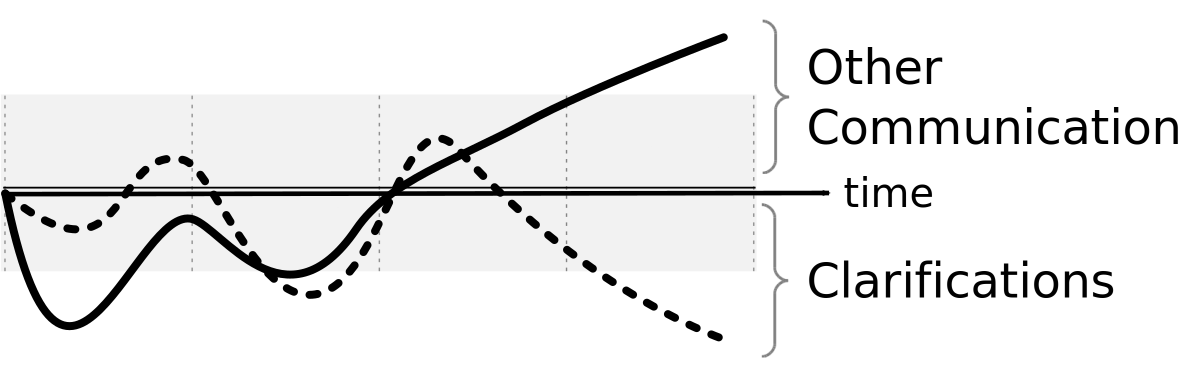
\includegraphics[width=0.7\columnwidth]{img/basic-pattern}
%\caption{Two different trajectories of reqts. communication}
%Predominance of clarifications in requirements-related communication may be problematic }
%\label{fig:basic-pattern}
%\end{center}
%\end{figure}

%Studying recorded online communication fills this gap by offering the potential to reveal patterns of communication that correlate to problematic situations around requirements development. 
In this demo we present a novel tool for analyzing online communication that helps managers to visualize the progression of clarification communication relative to other communication related to a particular requirement, thus providing support to differentiating between healthy and problematic requirements in the project. 
%Our \viss\ tool helps managers to analyze the content of stakeholder communication about  a particular requirement, identify specific instances of \emph{clarifying} communication, and examine the trajectory of clarifications (i.e. amount and progression) throughout the lifetime of a requirement. 
%Figure \ref{fig:basic-pattern} shows two distinct and quite different possible trajectories of \emph{clarifying} communication in the lifetime of a requirement. 
%While one would expect clarification to diminish as development of a requirement nears the end (solid line trajectory), its predominance throughout the requirement's life may be indicative of problematic requirements (dashed line trajectory). 
%The method proposed in this paper aims to identify these patterns automatically so that managers or involved stakeholders can be made aware of requirements that should be closely investigated.
\viss\ also visualizes stakeholder social networks related to a particular requirement to support the identification of communication breakdowns and experts for given topics.

%Figure \ref{fig:basic-pattern} depicts the characteristics of clarification communication related to a requirement (here: a story in Jazz).


%The contribution of this paper is the method for the detection and classification of clarification communication patterns, as well as a set of six communication patterns that we identified by applying our method in a large industrial project. 
%The remainder of the paper is structured as follows: Section \ref{sec:relatedwork} surveys related work in the study of communication in requirements engineering (RE), as well as related to information retrieval and automated classification techniques in RE. 
%Section \ref{sec:approach} introduces our research approach in studying requirements communication and the set of our techniques for the detection and classification of clarification  patterns. 
%We then describe the details of the industrial case study in which we applied our techniques in Sections \ref{sec:classification}, \ref{sec:visualization-and-patterns}, \ref{sec:recommendations} and \ref{sec:discussion}, and 
%give a detailed description of the three primary phases of our method: \emph{classification of requirements discussions}, \emph{clarification patterns development} and  \emph{pattern classification}.  
% conclude with future research steps in Section \ref{sec:conclusion}.

%\subsection{Background}
%The Jazz team uses Jazz as collaboration platform. It is the goal of the team to capture the entire communication in comments to \emph{workitems}. One of the workitem types, the \emph{story} contains requirements. Jazz follows an agile development approach, i.e. stories are refined during the project. This includes the decomposition in sub-workitems, most often of the workitem-type \emph{task}. 

%For a given requirement, the graph shows how the amount of clarification changes over time. 
%The example in the figure shows  a reoccurring characteristic that follows one of our six clarification communication patterns: the \emph{perfect clarification} pattern.


%Online communication to perform requirements related activities, such as elicitation, negotiation or development of requirements, is a critical part of large modern software projects. 
%Stakeholders in today's large software projects, most often at geographically distributed sites, largely rely on online communication in their collaboration. 
%Whether they follow an iterative discovery of requirements as in agile projects \cite{Cao2008}, or the time zone differences between stakeholders are too great to allow for frequent synchronous interaction (ref)2, or follow processes that mandate the recording of requirements communication online (ref3), these stakeholders perform various Requirements Engineering related activities through online communication. 

We conducted a preliminary evaluation in two ways. Firstly, we evaluated \viss's ability to correctly identify communication instances concerned with clarification and it's ability to derive meaningful visualizations of the clarification trajectory \cite{Knauss2012f}. 
Secondly, we showed  \viss's visualizations to software managers and asked them, whether the visualization was useful, if it did offer information they would have missed otherwise, and what actions they would perform based on the feedback, if any. 
This feedback lead to the development of additional features, e.g. social network analysis.

\begin{figure*}
\centering
\includegraphics[width=0.8\textwidth]{img/vissuelizer-screenshot}
\caption{The main window of the \viss\ shows a list of requirements (e.g. user stories in an issue tracker) and their clarification trajectories.}
\label{fig:screenshot}
\end{figure*}
% !TEX root = knauss-vissuelizer.tex
\section{Background and Related Work}
\todo[inline]{Define "Online Communication" = ticket system, issue tracker, task management system}
\todo[inline]{Use consistent terminology}

\todo[inline]{Harvest RE paper}

Since \todo{\footnotesize Read this, change text} tasks crosscut both the technical aspects of collaboration an communication, finding the right tasks at the right time is crucial to the success of a project \cite{Kraut1995}.
Treude and Storey identified the lack of visualizations as one of the most important short comings of today's task management systems \cite{Treude2010}. They also found that dashboards that report on the state of a task management system can become pivotal to task prioritization in critical project phases.

Ellis \todo{\footnotesize Read this, change text} et al. \cite{Ellis2007} report results from interviews of how developers use Bugzilla, a popular task management system. 
The motivation for their study was the design of a visualization tool for tasks. 
One of their key findings was that Bugzilla played a key role in managing the project. 
Their visualization reveals social and historical patterns in tasks, but it does not focus on exploration activities.

Many related studies focus on mining and analyzing quantitative data to reveal information about the evolution of the system or to predict future behaviours but only few works are concerned with visualizing and exploring this information space. 
Treude et al. \cite{Treude2012} present the workitemexplorer, a highly related tool that allows to explore the information stored in a task management system.
Compared to this work, \viss allows the analysis of a very specialized aspect, i.e. the analysis of online communication related to clarification of requirements. 
% !TEX root = knauss-vissuelizer.tex
\section{V:Issue:lizer}


\viss \footnote{Source code available at \url{https: //github.com/oerich/ReqtDisc}} is an interactive tool that allows software developers and managers to dynamically explore the discussion of requirements  in online repositories with a focus on highlighting the difference between clarification and implementation related communication.


The main window shows a list of requirements on the  left \todo{\footnotesize move to conclusion: (e.g. workitems in jazz, items in jira, issues in other systems)} (see Figure \ref{fig:screenshot}).
\viss\ adds visualizations to the selected discussions in the centre or in an extra window. 
These visualizations help to assess the communication through discussion events (e.g. comments) that are related to these requirements.
The panel on the right allows users to adjust parameters of the visualization.
Most importantly, the resolution of time intervals for the visualization can be adjusted, either as a fixed number of intervals (here: three and eight intervals), or as a fixed time interval (e.g. days, weeks, month).
%
\viss\  offers  two visualizations: 

\subsubsection{Clarification Trajectories} 
This visualization shows how the percentage of clarification events to other discussion events related to a requirement changes over its lifetime.
\begin{figure}[b]
\centering
\includegraphics[width=0.51\columnwidth]{img/example-trajectory}
\caption{Example of a requirements discussion's clarification trajectory}
\label{fig:example-trajectory}
\end{figure}
Since the visualization of the clarification trajectory (see Figure \ref{fig:example-trajectory}) is a new concept, it needs some explanation.
The black line represents the lifetime of the requirement discussion from the creation of the requirement in the system to the last recorded discussion event.
Dashed lines divide the lifeline into quarters and help to locate in which part of the lifetime discussion occurs.
Discussion events are depicted by rectangles that are shown below the lifeline if they are clarification events, and above the lifeline if they are not.
A grey line shows the sum of clarification.
In a classic trajectory with clarification up-front and only implementation related communication in the end, this grey line will start in the bottom left corner and raise to the upper right corner.
% For increased readability, the different types of discussion events are coloured in the tool (clarification events: red, other: blue).
\viss\ currently uses a Bayesian classifier to identify clarification events, i.e. a supervised machine learning algorithm.
Based on this classification, \viss\ generates trajectories and identifies reoccurring patterns (\emph{textbook-example, indifferent, discordant, procrastination, back-to-draft, and happy-ending}) \cite{Knauss2012f}.
Typically, there are many requirements without pathological findings, e.g. user stories with some clarification in the beginning and other communication events later on that show progress.
More suspicious trajectories show large amounts of clarification late in the iteration, perhaps even after the issue seemed to be solved. Others show no clarification at all, even though the requirement seems to be complex.
\subsubsection{Social Networks} 
This visualization shows the communication pattern of those participating in a requirement's discussion. 
The developers are presented as nodes and connections between nodes are weighted by the amount of communication both developers share about the requirement in a specific time interval (as defined above) in a requirement's lifetime. 
Thus, subgraphs of the contributors to the discussion in each time interval are created.
Two subgraphs are connected if  stakeholders appear in several time intervals. 
%Note that subgraphs can be matched to specific time intervals (here: three) where all actors of the subgraph communicate. 
%The interval can be a either a either a fixed number (here: three intervals), or a fixed time interval (e.g. days, weeks, month). 
\viss\ also displays the developer node as a pie chart to show the percentage of clarification vs. implementation-related communication in which the developer is involved (as highlighted in Figure \ref{fig:example-sn-large}).




% integrates information of the automatic analysis of online communication into the social networks, i.e. showing a pie chart with the percentage of clarification and implementation related communication for this developer.


% !TEX root = knauss-vissuelizer.tex
\section{Example Scenarios}
In this section we describe examples that highlight the functionality of the \viss tool.

\subsection{Where are the hotspots in a set of issues?}
\begin{figure}[b]
\includegraphics[width=\columnwidth]{img/example-trajectory}
\caption{Example of a clarification trajectory}
\label{fig:example-trajectory}
\end{figure}
Often, a clear understanding of requirements only evolves during the development of software.
This is especially true (but not limited to) agile software projects, where managers decide to frame only rudimentary requirements and refine the details on the go.
For a manager, it is important to know when problematic requirements surface, because they can have a serious impact on the project.
\viss helps managers in this scenario as follows:
\begin{enumerate}
\item The manager loads a set of issues (e.g. user stories for the current iteration).
\item \viss automatically analyzes the comments that are related to these issues and that are available in online communication.  
\item \viss creates a set of \emph{clarification trajectories} (c.f. Figure \ref{fig:example-trajectory}), one for each issue. 
Comments that are concerned with clarifying requirements are depicted by red rectangles below the timeline, other comments are depicted by blue rectangles above the timeline.
\item \viss also displays suggestive pattern names for distinctive trajectories (e.g. textbook-example, back-to-draft, procrastination).
\item The manager scrolls through the issues and associated trajectories and decides based on this rich information where to invest more resources.
\end{enumerate}
Typically, there is a number of issues without pathological findings, e.g. user stories with some clarification in the beginning and other communication events later on that show progress. But there are also suspicious trajectories: a large amount of clarification late in the iteration, perhaps even after the issue seemed to be solved. 
Or no clarification at all, even though the issue seems to be complex.

\subsection{Are there any communication breakdowns?}
After identifying those hotspots, the manager most likely wants to continue with a closer investigation. 
Often, he or she will investigate who participates in a discussion of an issue and who is not.
\viss helps managers in this scenario by creating social networks for an issue or a set of issues on the fly.
More over, \viss also integrates information of the automatic analysis of online communication into these social networks, i.e. showing for each actor the percentage of clarification and other communication.
Figure \ref{fig:example-sn} shows an example of an social network for the issue presented in Figure \ref{fig:example-trajectory}. 
\begin{figure}
\includegraphics[width=\columnwidth]{img/example-sn}
\caption{Example of a social network}
\label{fig:example-sn}
\end{figure}
The developers are presented as nodes (here: anonymized), and connections between nodes are weighted by the amount of communication both developers share about a given issue in a specific time interval. 
In the example above, the manager might conclude that there is no single person who is coordinating the work around this issue, because there is no actor who participates in all relevant time intervals.
A suitable action might be to assign the responsibility to a more experienced developer.

\subsection{Who is knowledgeable about a given topic?}

Integrating the right persons in the loop for an important feature is a crucial ability for managers.
To support managers in this task, \viss distinguishes between two types of knowledge: domain knowledge that shows in communication events related to clarification and technical knowledge that shows in other communication events.
In order to leverage the power of \viss for this task, the manager selects a number of issues that are related to a given topic. 
\viss integrates the social networks of these issues in a single large network (see Figure \ref{fig:example-sn-large}).
\begin{figure}
\includegraphics[width=\columnwidth]{img/example-sn-large}
\caption{Example of a social network of a set of issues}
\label{fig:example-sn-large}
\end{figure}
The manager looks for candidates with a balanced percentage of clarification and other communication and a medium centrality, actors with high centrality might already have a very high workload.

% !TEX root = knauss-vissuelizer.tex
\section{Preliminary Evaluation}
\todo[inline]{RE Paper}
\todo[inline]{IBM Interviews}
\todo[inline]{VIATEC Software Management Round Table}
%\input{recommendations}
%\input{discussion}
% !TEX root = knauss-vissuelizer.tex
\section{Conclusion and Future Work}
\todo[inline]{Dana, please review conclusion}
 \viss\ is a visualization tool to analyze requirements clarification in online communication in a project.
Especially agile and distributed projects demand such analysis: agile projects often only sketch requirements in sufficient detail to plan the next iteration and leave the details to be clarified during the development.
Without the ability to measure how this clarification diminishes over time and especially before feature delivery, managers find it hard to manage project risks during iterations.
Our preliminary evaluation has shown that our visualizations allow managers to identify hotspots, e.g. user stories that are not clear to the team. 
Furthermore, \viss\ supports managers in investigating the cause of those hotspots and in identifying suitable actions to disarm problematic or risky situations where the team has insufficient understanding of requirements.
 
In future work, we will evaluate how practitioners use our tool in their daily work. 
This will help us to gain further insight on how managers can use information about requirements clarification over time and to quantify the benefits that tools like the \viss\ can offer.

Such further evaluation should also relate features of online communication (i.e. network centrality, late clarification, no clarification) with typical problems of requirements related discussions, such as feature creep \cite{Jones1996} or symmetry of ignorance \cite{Fischer2000}.

This paper has a complementary video at \url{http://www.youtube.com/watch?v=Oy3xvzjy3BQ&feature=youtu.be}. In addition, the source code of the tool is available at \url{https://github.com/oerich/ReqtDisc}.
\section*{Acknowledgements}
\todo[inline]{There is a number of people we should acknowledge.}
%\vspace{-1cm}
\balance

% \listoftodos

\bibliographystyle{IEEEtran}
\bibliography{IEEEabrv,bibliography}
\end{document}
